
\subsection{Rapid Tests}
\label{subsec:appendix_rapid_tests}

\begin{figure}[ht] % Share tested per day
  \centering
  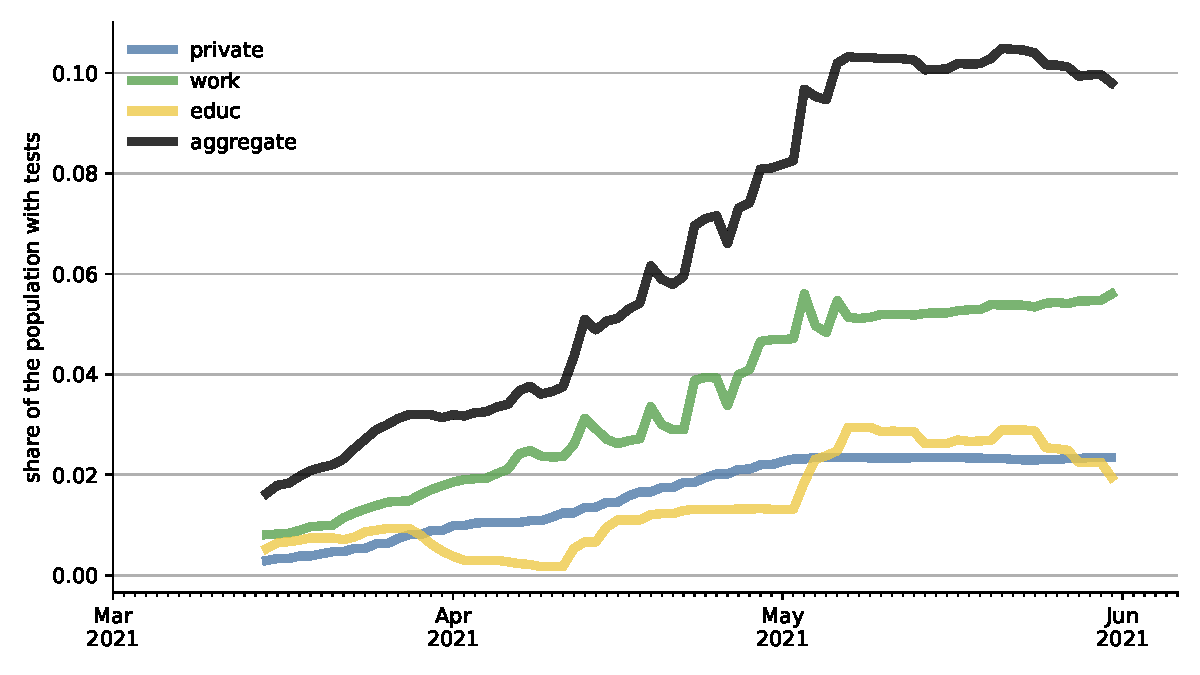
\includegraphics[width=\textwidth]{figures/results/figures/rapid_test_statistics/popshare_tested}
  \caption{Share of the Population Demanding a Rapid Test Because of Different Channels
  on a Given Day}
  \label{fig:rapid_test_demand_by_channel}
  \floatfoot{\noindent \textit{Note:}
    Rapid tests in the education setting are demanded by teachers (nursery, preschool and
    school) as well as school pupils. After Easter the required frequency of tests is
    increased from once per week to twice per week. Work rapid tests are demanded by
    individuals that still have work contacts, i.e. do not work from home. The share of
    employers offering rapid tests increases over the time frame and the frequency of
    testing is also increased. Tests are demanded by individuals for one of three private
    reasons: having developed symptoms without access to a PCR test, having a household
    member that has tested positive or developed symptoms or having planned weekly
    meeting with friends. }
\end{figure}


\begin{figure}   % Number of True Positive / False Positive / True Negative / False Negative
    \centering
    \begin{subfigure}[b]{0.425\textwidth}
        \centering
        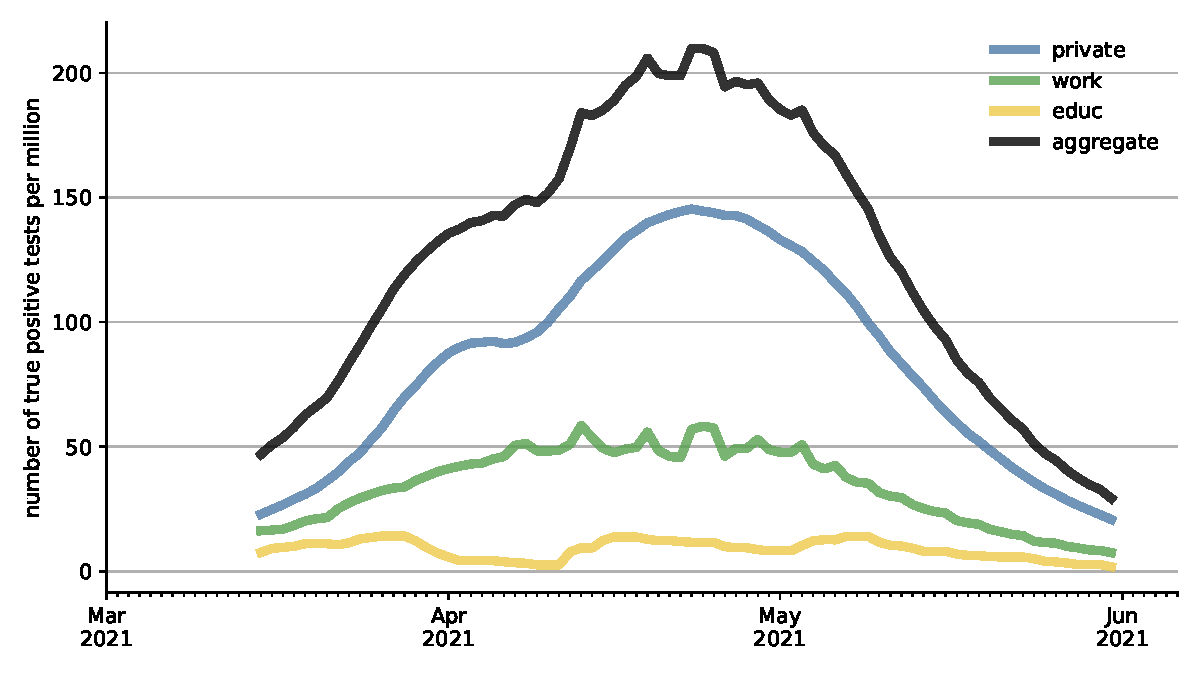
\includegraphics[width=\textwidth]{figures/results/figures/rapid_test_statistics/number_true_positive}
        \caption{Number of Discovered Cases Due to Rapid Tests by Channel}
        \label{fig:rapid_tests_number_true_positive}
    \end{subfigure}
    \hfill
    \begin{subfigure}[b]{0.425\textwidth}
        \centering
        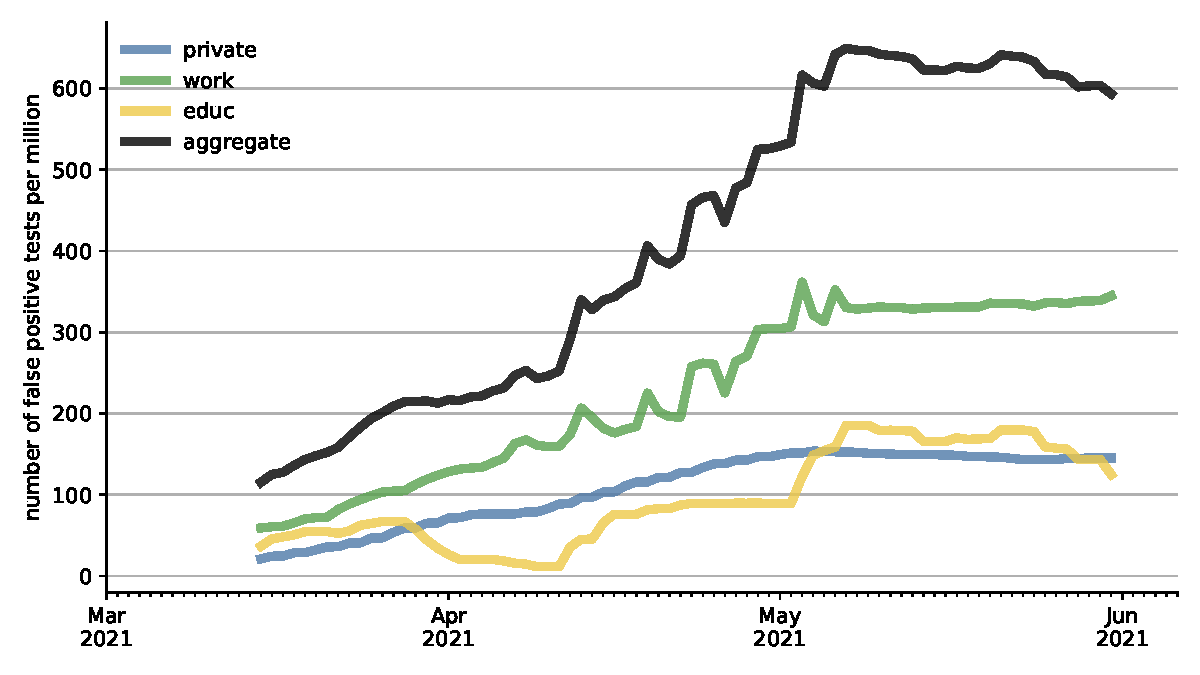
\includegraphics[width=\textwidth]{figures/results/figures/rapid_test_statistics/number_false_positive}
        \caption{Number of False Positive Rapid Tests by Channel}
        \label{fig:rapid_tests_number_false_positive}
    \end{subfigure}
    \vskip3ex
    \begin{subfigure}[b]{0.425\textwidth}
        \centering
        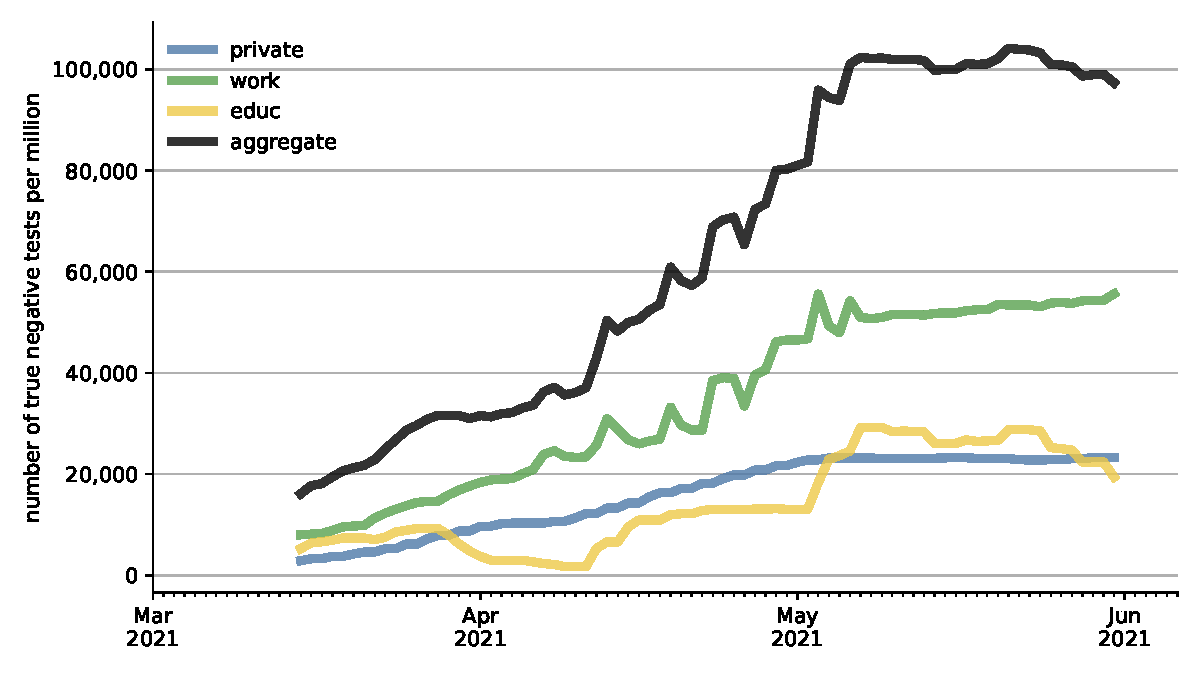
\includegraphics[width=\textwidth]{figures/results/figures/rapid_test_statistics/number_true_negative}
        \caption{Number of True Negative Rapid Tests by Channel}
        \label{fig:rapid_tests_number_true_negative}
    \end{subfigure}
    \hfill
    \begin{subfigure}[b]{0.425\textwidth}
        \centering
        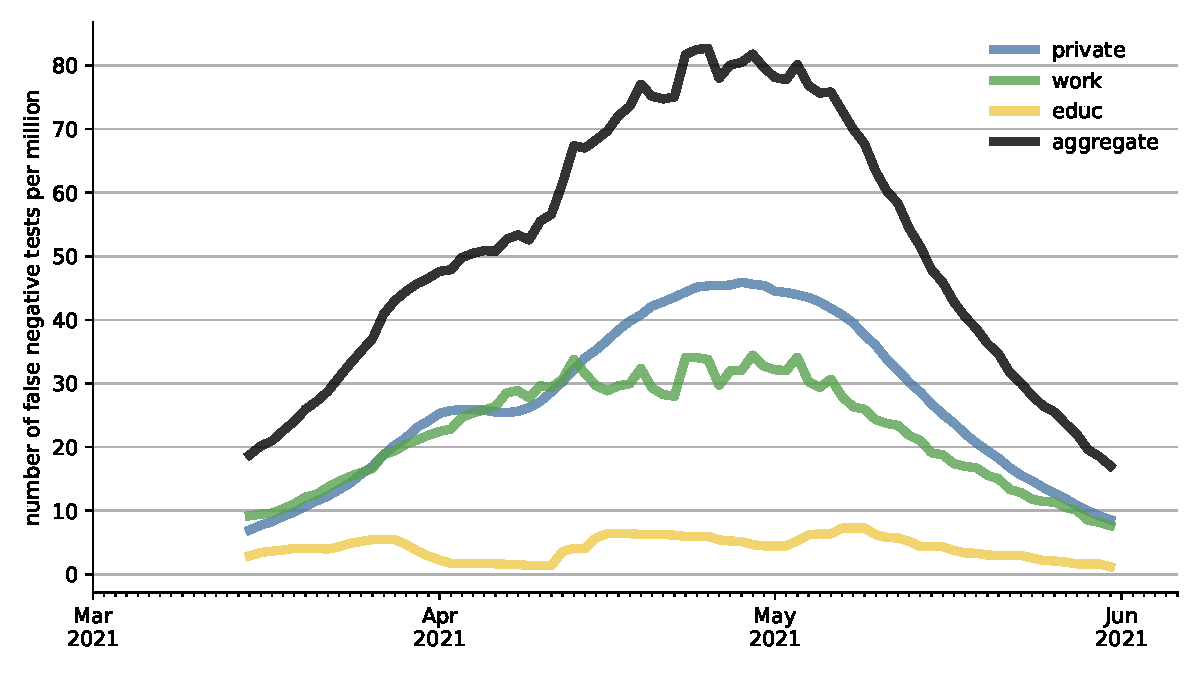
\includegraphics[width=\textwidth]{figures/results/figures/rapid_test_statistics/number_false_negative}
        \caption{Number of False Negative Rapid Tests by Channel}
        \label{fig:rapid_tests_number_false_negative}
    \end{subfigure}
    \vskip3ex
    \caption{Rapid Test Results}
    \label{fig:rapid_test_results_numbers}

    \floatfoot{\noindent \textit{Note:}
      The number of rapid tests of each category are upscaled to the full German
      population. \textcolor{red}{To be written.}
    }
\end{figure}


\begin{figure} % True Positive / False Positive / True Negative / False Negative Rate
    \centering
    % \begin{subfigure}[b]{0.425\textwidth}
    %     \centering
    %     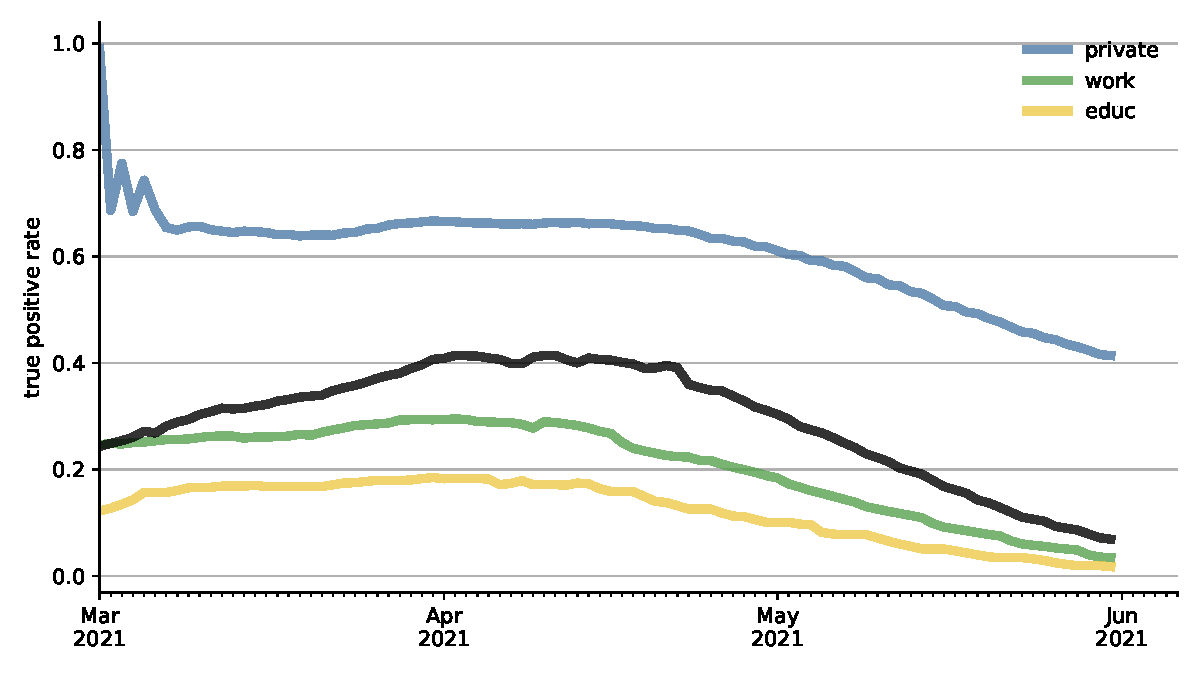
\includegraphics[width=\textwidth]{figures/results/figures/rapid_test_statistics/true_positive_rate}
    %     \caption{Rate of True Positive Rapid Tests by Channel}
    %     \label{fig:rapid_tests_true_positive_rate}
    % \end{subfigure}
    % \hfill
    \begin{subfigure}[b]{0.425\textwidth}
        \centering
        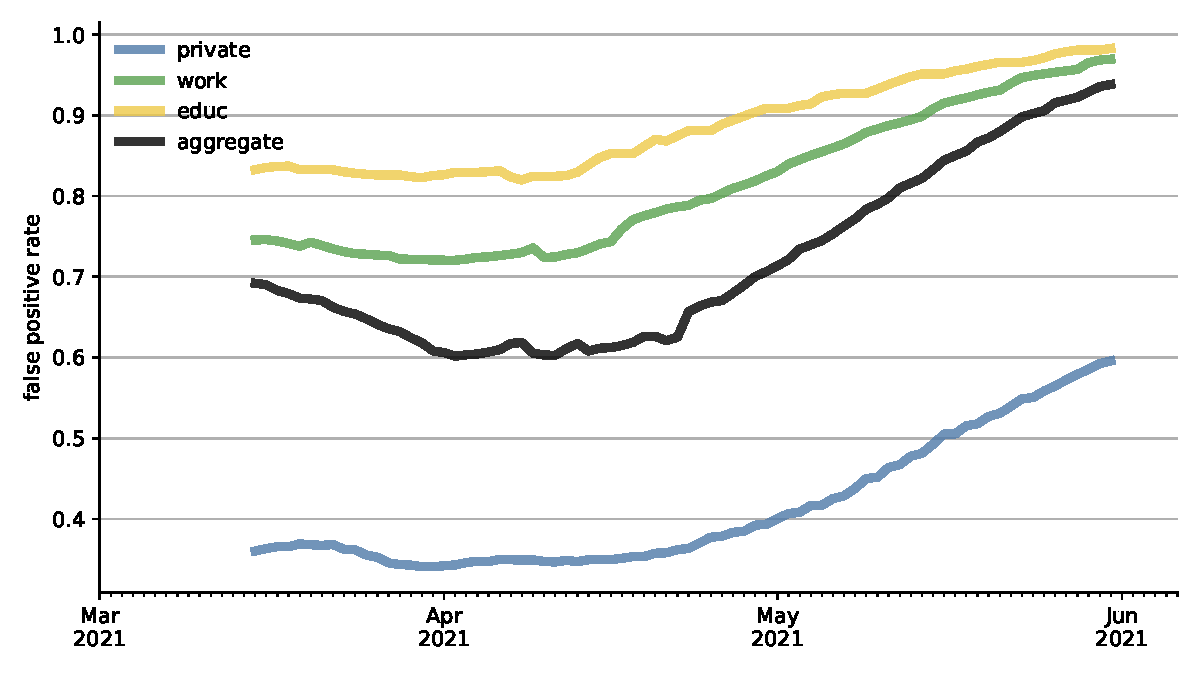
\includegraphics[width=\textwidth]{figures/results/figures/rapid_test_statistics/false_positive_rate}
        \caption{Rate of False Positive Rapid Tests by Channel}
        \label{fig:rapid_tests_false_positive_rate}
    \end{subfigure}
    % \vskip3ex
    % \begin{subfigure}[b]{0.425\textwidth}
    %     \centering
    %     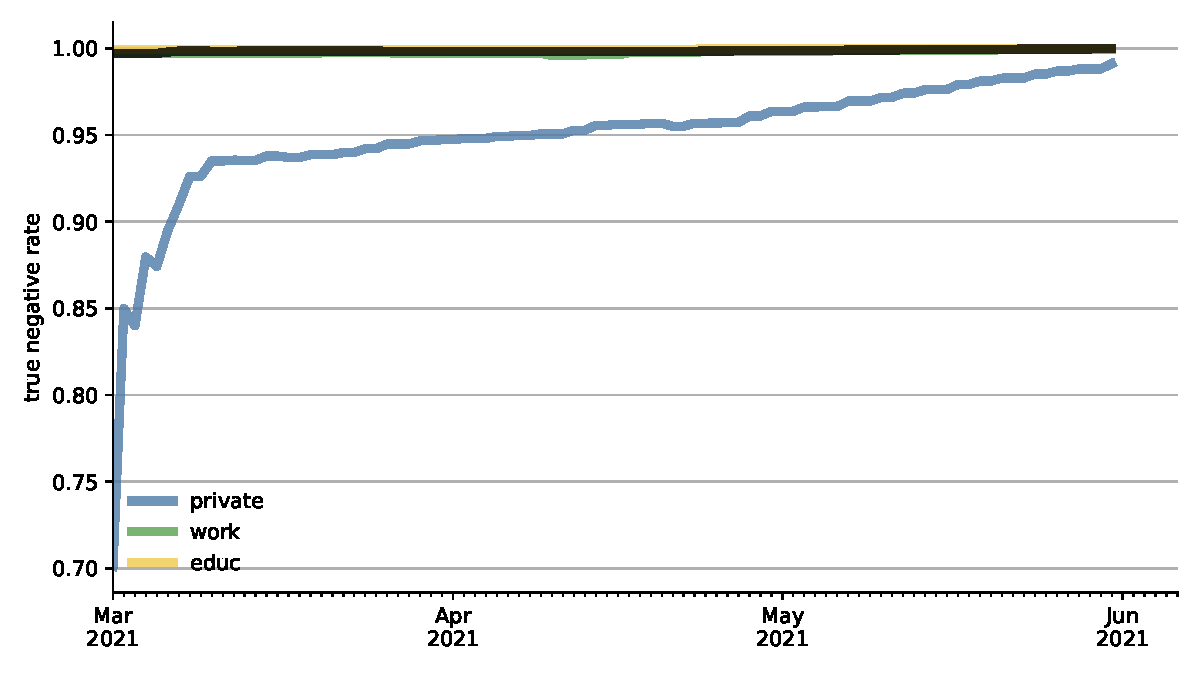
\includegraphics[width=\textwidth]{figures/results/figures/rapid_test_statistics/true_negative_rate}
    %     \caption{Rate of True Negative Rapid Tests by Channel}
    %     \label{fig:rapid_tests_true_negative_rate}
    % \end{subfigure}
    \hfill
    \begin{subfigure}[b]{0.425\textwidth}
        \centering
        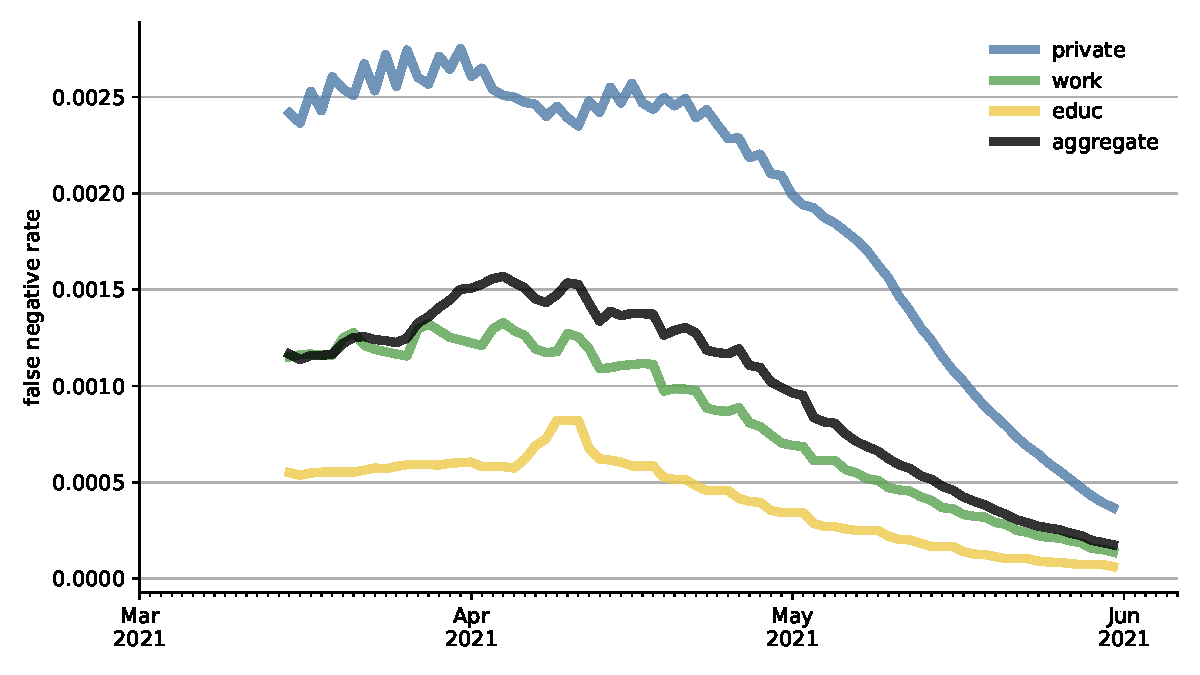
\includegraphics[width=\textwidth]{figures/results/figures/rapid_test_statistics/false_negative_rate}
        \caption{Rate of False Negative Rapid Tests by Channel}
        \label{fig:rapid_tests_false_negative_rate}
    \end{subfigure}
    \vskip3ex
    \caption{Rapid Test Rates by Channel}
    \label{fig:rapid_test_results_rates}

    \floatfoot{\noindent \textit{Note:}
      \textcolor{red}{To be written.}
    }
\end{figure}

\begin{figure} % Share of Tests That Are True Positive / False Positive / True Negative / False Negative
    \centering
    \begin{subfigure}[b]{0.425\textwidth}
        \centering
        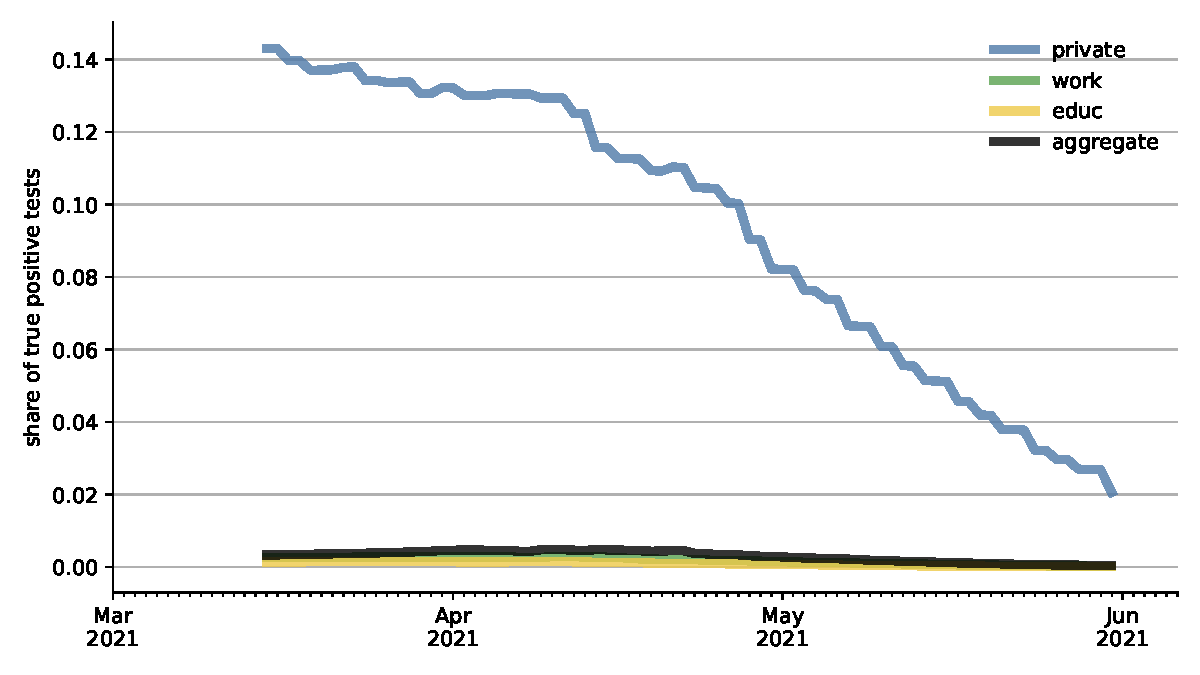
\includegraphics[width=\textwidth]{figures/results/figures/rapid_test_statistics/testshare_true_positive}
        \caption{Share of Tests That Are True Positive by Channel}
        \label{fig:rapid_tests_testshare_true_positive}
    \end{subfigure}
    \hfill
    \begin{subfigure}[b]{0.425\textwidth}
        \centering
        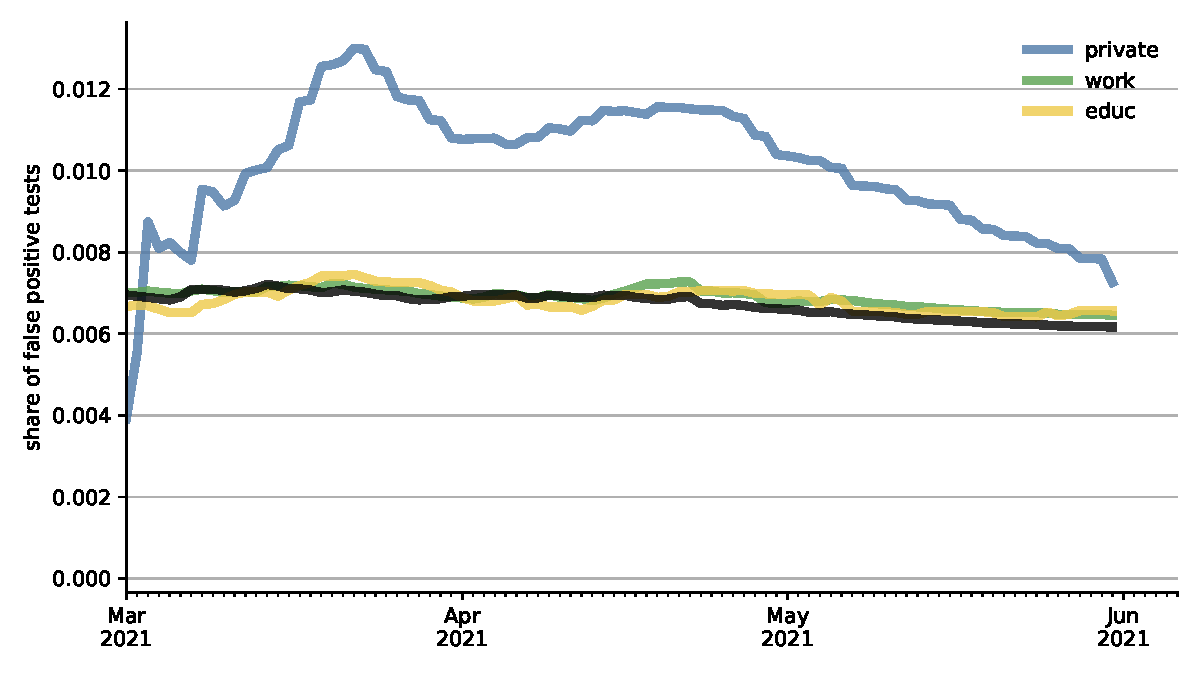
\includegraphics[width=\textwidth]{figures/results/figures/rapid_test_statistics/testshare_false_positive}
        \caption{Share of Tests That Are False Positive by Channel}
        \label{fig:rapid_tests_testshare_false_positive}
    \end{subfigure}
    \vskip3ex
    \begin{subfigure}[b]{0.425\textwidth}
        \centering
        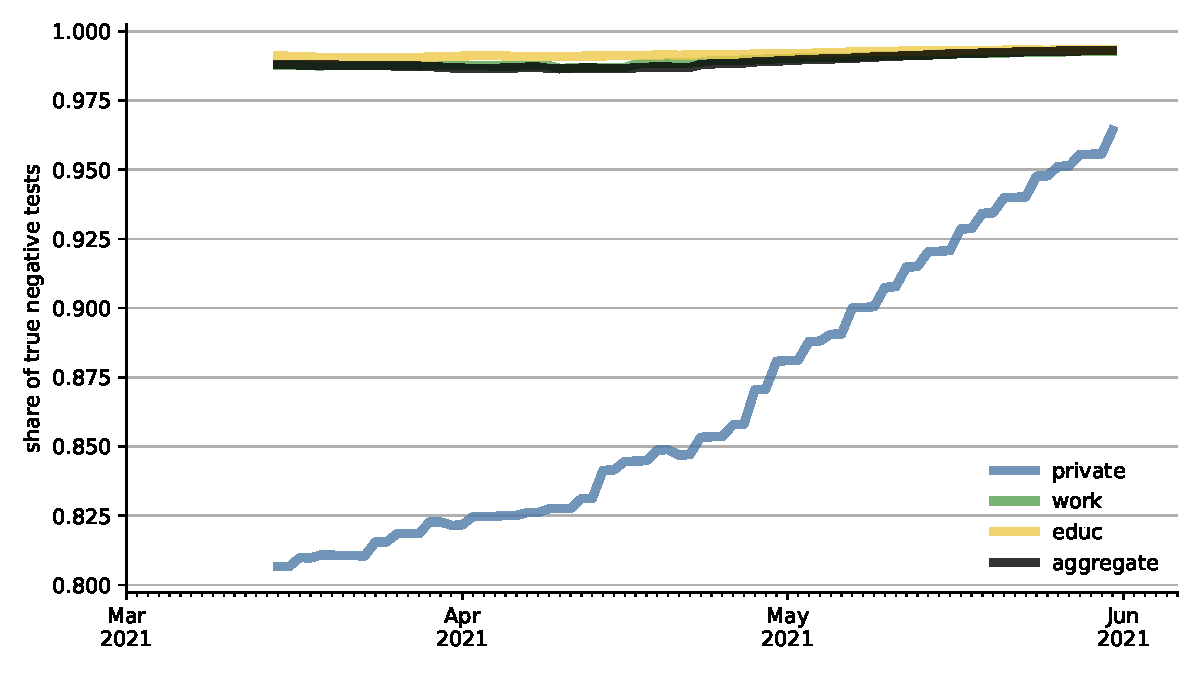
\includegraphics[width=\textwidth]{figures/results/figures/rapid_test_statistics/testshare_true_negative}
        \caption{Share of Tests That Are True Negative by Channel}
        \label{fig:rapid_tests_testshare_true_negative}
    \end{subfigure}
    \hfill
    \begin{subfigure}[b]{0.425\textwidth}
        \centering
        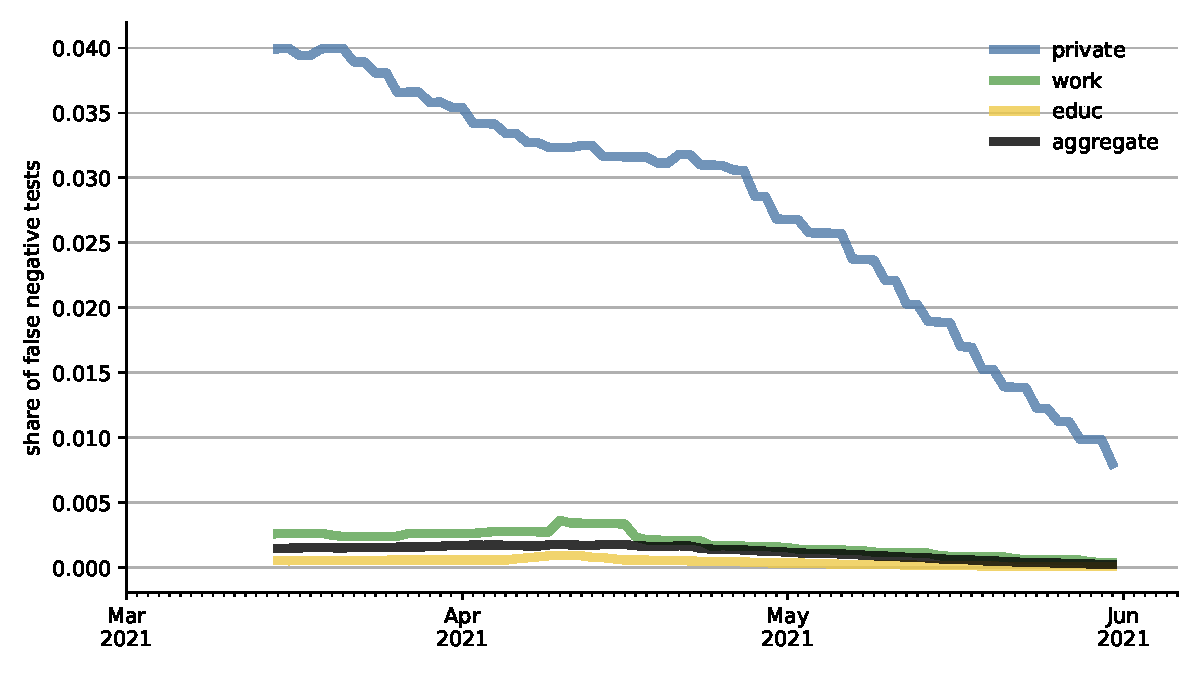
\includegraphics[width=\textwidth]{figures/results/figures/rapid_test_statistics/testshare_false_negative}
        \caption{Share of Tests That Are False Negative by Channel}
        \label{fig:rapid_tests_testshare_false_negative}
    \end{subfigure}
    \vskip3ex
    \caption{Share of Rapid Tests by Outcome and True Infection Status}
    \label{fig:rapid_test_results_test_shares}

    \floatfoot{\noindent \textit{Note:}
      \textcolor{red}{To be written.}
    }
\end{figure}






\FloatBarrier